\documentclass[dvips, lscape]{foils}
%\documentclass[dvips, french]{slides}
\textwidth 19cm
\textheight 25cm 
\topmargin -1cm 
\oddsidemargin  -1.5cm 
\evensidemargin  -1.5cm

% Maths
\usepackage{amsfonts, amsmath, amssymb}
% \newcommand{\Acal}{\mathcal{A}}
% \newcommand{\Ccal}{\mathcal{C}}

\newcommand{\coefbin}[2]{\left( 
    \begin{array}{c} #1 \\ #2 \end{array} 
  \right)}
\newcommand{\Dcal}{\mathcal{D}}
\newcommand{\Ecal}{\mathcal{E}}
\newcommand{\Ncal}{\mathcal{N}}
% \newcommand{\Pcal}{\mathcal{P}}
% \newcommand{\Ucal}{\mathcal{U}}om
\newcommand{\Hbf}{{\bf H}}
\newcommand{\Bcal}{\mathcal{B}}
\newcommand{\Lcal}{\mathcal{L}}
\newcommand{\Tcal}{\mathcal{T}}
\newcommand{\Ucal}{\mathcal{U}}
\newcommand{\alphabf}{\mbox{\mathversion{bold}{$\alpha$}}}
\newcommand{\betabf}{\mbox{\mathversion{bold}{$\beta$}}}
\newcommand{\gammabf}{\mbox{\mathversion{bold}{$\gamma$}}}
\newcommand{\psibf}{\mbox{\mathversion{bold}{$\psi$}}}
\newcommand{\taubf}{\mbox{\mathversion{bold}{$\tau$}}}
\newcommand{\Rbb}{\mathbb{R}}
\newcommand{\Sbf}{{\bf S}}
% \newcommand{\bps}{\mbox{bps}}
\newcommand{\ubf}{{\bf u}}
\newcommand{\vbf}{{\bf v}}
\newcommand{\Esp}{{\mathbb E}}
% \newcommand{\Var}{{\mathbb V}}
\newcommand{\Indic}{{\mathbb I}}
\newcommand{\liste}{$\bullet \quad$}
\newcommand{\lFDR}{\ell FDR}

% Couleur et graphiques
\usepackage{color}
\usepackage{graphics}
\usepackage{epsfig} 
\usepackage{pstcol}

% Texte
\usepackage{lscape}
\usepackage{../../../../Latex/fancyheadings, rotating, enumerate}
%\usepackage[french]{babel}
\usepackage[latin1]{inputenc}
\definecolor{darkgreen}{cmyk}{0.5, 0, 0.5, 0.5}
\definecolor{orange}{cmyk}{0, 0.6, 0.8, 0}
\definecolor{jaune}{cmyk}{0, 0.5, 0.5, 0}
\newcommand{\textblue}[1]{\textcolor{blue}{#1}}
\newcommand{\textred}[1]{\textcolor{red}{#1}}
\newcommand{\textgreen}[1]{\textcolor{green}{ #1}}
\newcommand{\textlightgreen}[1]{\textcolor{green}{#1}}
%\newcommand{\textgreen}[1]{\textcolor{darkgreen}{#1}}
\newcommand{\textorange}[1]{\textcolor{orange}{#1}}
\newcommand{\textyellow}[1]{\textcolor{yellow}{#1}}

% Sections
\newcommand{\chapter}[1]{\centerline{\Large \textblue{#1}}}
\newcommand{\section}[1]{\centerline{\large \textblue{#1}}}
\newcommand{\subsection}[1]{\noindent{\large \textblue{#1}}}
\newcommand{\paragraph}[1]{\noindent {\textblue{#1}}}

%%%%%%%%%%%%%%%%%%%%%%%%%%%%%%%%%%%%%%%%%%%%%%%%%%%%%%%%%%%%%%%%%%%%%%
%%%%%%%%%%%%%%%%%%%%%%%%%%%%%%%%%%%%%%%%%%%%%%%%%%%%%%%%%%%%%%%%%%%%%%
%%%%%%%%%%%%%%%%%%%%%%%%%%%%%%%%%%%%%%%%%%%%%%%%%%%%%%%%%%%%%%%%%%%%%%
%%%%%%%%%%%%%%%%%%%%%%%%%%%%%%%%%%%%%%%%%%%%%%%%%%%%%%%%%%%%%%%%%%%%%%
\begin{document}
%%%%%%%%%%%%%%%%%%%%%%%%%%%%%%%%%%%%%%%%%%%%%%%%%%%%%%%%%%%%%%%%%%%%%%
%%%%%%%%%%%%%%%%%%%%%%%%%%%%%%%%%%%%%%%%%%%%%%%%%%%%%%%%%%%%%%%%%%%%%%
%%%%%%%%%%%%%%%%%%%%%%%%%%%%%%%%%%%%%%%%%%%%%%%%%%%%%%%%%%%%%%%%%%%%%%
%%%%%%%%%%%%%%%%%%%%%%%%%%%%%%%%%%%%%%%%%%%%%%%%%%%%%%%%%%%%%%%%%%%%%%
\landscape
\headrulewidth 0pt 
\pagestyle{fancy} 
\cfoot{}
\rfoot{\begin{rotate}{90}{
      \hspace{1cm} \tiny S. Robin: Semi-parametric mixture model
      }\end{rotate}}
\rhead{\begin{rotate}{90}{
      \hspace{-.5cm} \tiny \thepage
      }\end{rotate}}

%%%%%%%%%%%%%%%%%%%%%%%%%%%%%%%%%%%%%%%%%%%%%%%%%%%%%%%%%%%%%%%%%%%%%%
%%%%%%%%%%%%%%%%%%%%%%%%%%%%%%%%%%%%%%%%%%%%%%%%%%%%%%%%%%%%%%%%%%%%%%

~
\vspace{2cm}
\begin{center}
  \chapter{A semi parametric approach for mixture models: }
  \bigskip
  \chapter{Application to FDR and local FDR} 
  \bigskip

   \vspace{1cm}
   {\large S. {Robin},  J.-J. {Daudin}, A. {Bar-Hen}, L. {Pierre}} \\
   robin@inapg.inra.fr

   {UMR INA-PG / INRA, Paris} \\
   {Math�matique et Informatique Appliqu�es}
   
   \vspace{2cm}
   {INSERM Workshop, October 2005}
\end{center}

%%%%%%%%%%%%%%%%%%%%%%%%%%%%%%%%%%%%%%%%%%%%%%%%%%%%%%%%%%%%%%%%%%%%%%
%%%%%%%%%%%%%%%%%%%%%%%%%%%%%%%%%%%%%%%%%%%%%%%%%%%%%%%%%%%%%%%%%%%%%%
%%%%%%%%%%%%%%%%%%%%%%%%%%%%%%%%%%%%%%%%%%%%%%%%%%%%%%%%%%%%%%%%%%%%%%
%%%%%%%%%%%%%%%%%%%%%%%%%%%%%%%%%%%%%%%%%%%%%%%%%%%%%%%%%%%%%%%%%%%%%%
\newpage
\chapter{Multiple testing}
\bigskip
\centerline{\textblue{Ex: Differential analysis of microarray data}}

\paragraph{Elementary data:} $Y_{itr} = $ expression level of gene
$i$ in condition $t$ ($t=1$ or $2$) at replicate $r$

\paragraph{Differentially expressed genes} are genes for which
$Y_{i1r}$ is not distributed as $Y_{i2r}$. 

Null hypothesis for gene $i$:
$
\Hbf_0(i) = \{Y_{i1r} \overset{\Lcal}{=} Y_{i2r}\}
$

\paragraph{Statistical test:} Student, Wilcoxon, permutation, {\it
  etc.} 

For each gene we get:
$$
\begin{tabular}{ll}
  the value of the test statistic & $T_i$ \\
  \\
  the corresponding $p$-value & $P_i = \Pr\{\Tcal > T_i
  \;|\;\Hbf_0(i)\}$ 
\end{tabular}
$$
\paragraph{Comparing more than 2 conditions.} Same problem: Fisher,
Kruskall-Wallis tests provide one $p$-value for each gene.

\newpage
\section{Relation between $P_i$ and $T_i$} 

\vspace{.5cm}
The $p$-value is the probability for the test statistic $\Tcal$ to be larger
than the observed value $T_i$: 
$$
P_i = \Pr\{|\Tcal| > |T_i| \;|\;\Hbf_0(i)\}.
$$ \\
$$
\begin{pspicture}(20, 8.7)(0, -1.3)
  \rput[b](10, -2){ 
     \epsfig{figure=../Figures/pvalue-N01.ps, height=12cm, width=24cm, clip=}    
    }

  \rput[B](17.5, 1.5){$P_i/2$}
  %\psline[linewidth=0.1]{<-}(15, 0.8)(16.7, 3)

  \rput[B](3.5, 1.5){$P_i/2$}
  %\psline[linewidth=0.1]{<-}(5, 0.8)(3.5, 3)

  \rput[B](4.5, -0.6){$-|T_i|$}
  \rput[B](16.5, -0.6){$+|T_i|$}
\end{pspicture}
$$

%%%%%%%%%%%%%%%%%%%%%%%%%%%%%%%%%%%%%%%%%%%%%%%%%%%%%%%%%%%%%%%%%%%%%%
\newpage
\paragraph{Shape of the $p$-value histogram}

\begin{itemize}
\item Under $\Hbf_0$ (non-differentially expressed genes), $P_i$ is
uniformly distributed over $[0, 1]$. 
\item Otherwise (differentially expressed genes), $P_i$ has to be small.
\end{itemize}
So, the histogram of the $p$-values must look 
$$
\hspace{-.5cm}
\begin{tabular}{ccc}
  like this, & but not like this, & nor like this. \\ 
  \epsfig{figure=../Figures/HistoPvalRef.ps, height=8cm, width=8cm,
    clip=, bbllx=26, bblly=40, bburx=176, bbury=130} &  
  \epsfig{figure=../Figures/TDdiff.eps, height=8cm, width=8cm,
    clip=, bbllx=25, bblly=28, bburx=176, bbury=131} & 
  \epsfig{figure=../Figures/CompExcepLRT.eps, height=8cm, width=8cm,
    clip=, bbllx=108, bblly=663, bburx=509, bbury=730.5} 
\end{tabular}
$$
%%%%%%%%%%%%%%%%%%%%%%%%%%%%%%%%%%%%%%%%%%%%%%%%%%%%%%%%%%%%%%%%%%%%%%
%%%%%%%%%%%%%%%%%%%%%%%%%%%%%%%%%%%%%%%%%%%%%%%%%%%%%%%%%%%%%%%%%%%%%%
%%%%%%%%%%%%%%%%%%%%%%%%%%%%%%%%%%%%%%%%%%%%%%%%%%%%%%%%%%%%%%%%%%%%%%
\newpage
\section{False positives and false negatives}
\bigskip
%%%%%%%%%%%%%%%%%%%%%%%%%%%%%%%%%%%%%%%%%%%%%%%%%%%%%%%%%%%%%%%%%%%%%%
%%%%%%%%%%%%%%%%%%%%%%%%%%%%%%%%%%%%%%%%%%%%%%%%%%%%%%%%%%%%%%%%%%%%%%
%\section{General problem}

\paragraph{Rejection rule:} For a given level $\alpha$, 
$$
\begin{tabular}{rcl}
  $P_i < \alpha$ & $\qquad \Longrightarrow \qquad$ & gene $i$ is
    declared positive \\
  & & (i.e. differentially expressed)
\end{tabular}
$$

\paragraph{Multiple testing:} When performing $n$ simultaneous tests
$$
\begin{tabular}{c|cc|c}
  & \multicolumn{2}{c}{Decision (random)} & \\
  & $\Hbf_0$ accepted & $\Hbf_0$ rejected & \\
  \hline
  $\Hbf_0$ true 
  & \begin{tabular}{c} $TN$ \\ true negatives \end{tabular} 
  & \begin{tabular}{c} $FP$ \\ false positives \end{tabular}
  & \begin{tabular}{c} $n_0$ \\ negatives \end{tabular} \\
  $\Hbf_0$ false 
  & \begin{tabular}{c} $FN$ \\ false negatives \end{tabular} 
  & \begin{tabular}{c} $TP$ \\ true positives \end{tabular} 
  & \begin{tabular}{c} $n_1$ \\ positives \end{tabular} \\
  \hline
  & $N$ negatives & $R$ positives & $n$
\end{tabular}
$$
All the random quantities (capital) depend on the data and the
pre-fixed level $\alpha$.

\newpage
\paragraph{Microarray experiment:} Typically $n=10\;000$ tests are
performed simultaneously 

For $\alpha = 5\%$, if no gene is actually differentially expressed
($n_1 = 0, n_0 = n$), we expect
$$
0.05 \times 10\;000 = 500 \mbox{``positive'' genes}
$$
which are \paragraph{all false positives}.

\paragraph{Problem:} We'd like to control some ``global risk'' $\alpha^*$
such as 
\begin{itemize}
\item the probability of having one false positive (FWER)
  $$
  FWER = \Pr\{FP \geq 1\},
  $$
\item or the proportion of false positives (FDR)
  $$
  FDR = \Esp(FP/R).
  $$
\end{itemize}
(Benjamini \& Hochberg, JRSS-B, 1995; Dudoit \& al., Stat. Sci.,
2003)

%%%%%%%%%%%%%%%%%%%%%%%%%%%%%%%%%%%%%%%%%%%%%%%%%%%%%%%%%%%%%%%%%%%%%%
%%%%%%%%%%%%%%%%%%%%%%%%%%%%%%%%%%%%%%%%%%%%%%%%%%%%%%%%%%%%%%%%%%%%%%
  \newpage
\section{False Discovery Rate (FDR)}
% \bigskip
% \centerline{$FDR = \Esp(FP/R)$}

\paragraph{Idea:} Instead of preventing any error, just control the
proportion of errors 
\centerline{$\Longrightarrow$ less conservative}

\hspace{-2cm}
\begin{tabular}{ll}
  \begin{tabular}{p{14cm}}
    \paragraph{Benjamini \& Hochberg (95) procedure:} \\
    \\
    Given the sorted $p$-values \\
    $$P_{(1)} \leq \dots \leq P_{(i)} \leq \dots \leq P_{(n)}$$
    \\
    reject $\Hbf_0$ for all $(i)$ such as 
    $$P_{(i)} \leq \frac{i \alpha^*}n \quad \Longrightarrow \quad
    FDR \leq \frac{n_0}n \alpha^* \leq \alpha^*$$
  \end{tabular}
  &
  \begin{tabular}{l}
  \epsfig{figure=../Figures/HistoPvalRef.ps, height=10cm, width=10cm,
    clip=, bbllx=26, bblly=40, bburx=176, bbury=130}   
%     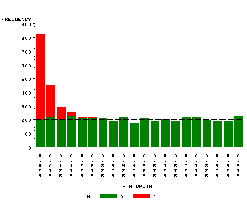
\epsfig{
%       file=.../Figures/HistoPvalRef.ps,
%       height=8cm, width=8cm, bbllx=82, bblly=304, bburx=277,
%       bbury=460, angle=90, clip=} 
  \end{tabular}
\end{tabular}


\paragraph{Benjamini \& Yakutieli (01):} For correlated
test statistics
$$
P_{(i)} \leq \frac{i \alpha^*}{n (\sum_j 1/j)}.
$$

%%%%%%%%%%%%%%%%%%%%%%%%%%%%%%%%%%%%%%%%%%%%%%%%%%%%%%%%%%%%%%%%%%%%%%
%%%%%%%%%%%%%%%%%%%%%%%%%%%%%%%%%%%%%%%%%%%%%%%%%%%%%%%%%%%%%%%%%%%%%%
\newpage
\paragraph{Number of positive genes} for $\alpha^* = 5\%$

\begin{tabular}{l}
  $p$-value: \\
  \qquad 1887 \\
  \\
  Bonferroni: \\
  \qquad 111 \\
  \\
  Sidak: \\
  \qquad 113 \\
  \\
  Holm: \\\\
  \qquad 112 \\
  \\
  Sidak adap.: \\
  \qquad 113 \\
  \\
  FDR: \\
  \qquad  903 \\
\end{tabular}
\begin{tabular}{l}
  \epsfig{figure=../Figures/Golub-adjp-zoom.eps, height=15cm, width=20cm,
    bbllx=64, bblly=209, bburx=550, bbury=590, clip}
\end{tabular}

%%%%%%%%%%%%%%%%%%%%%%%%%%%%%%%%%%%%%%%%%%%%%%%%%%%%%%%%%%%%%%%%%%%%%%
%%%%%%%%%%%%%%%%%%%%%%%%%%%%%%%%%%%%%%%%%%%%%%%%%%%%%%%%%%%%%%%%%%%%%%
\newpage
\chapter{Mixture model} 
%%%%%%%%%%%%%%%%%%%%%%%%%%%%%%%%%%%%%%%%%%%%%%%%%%%%%%%%%%%%%%%%%%%%%%
%%%%%%%%%%%%%%%%%%%%%%%%%%%%%%%%%%%%%%%%%%%%%%%%%%%%%%%%%%%%%%%%%%%%%%

%%%%%%%%%%%%%%%%%%%%%%%%%%%%%%%%%%%%%%%%%%%%%%%%%%%%%%%%%%%%%%%%%%%%%%
\bigskip
\section{Local False Discovery Rate}
%%%%%%%%%%%%%%%%%%%%%%%%%%%%%%%%%%%%%%%%%%%%%%%%%%%%%%%%%%%%%%%%%%%%%%

\noindent FDR provides a general information about the risk of the whole
procedure (up to step $i$). But we are actually interested in a
specific risk, associated to each gene.

\paragraph{Derivative of the FDR:} $\lFDR_{(i)}$ can be also defined as the
derivative of the FDR
$$
\lFDR(t) = \lim_{h \downarrow 0} \frac{FDR(t+h) - FDR(t)}{h}
$$
which can be estimated by 
$$
\widehat{n}_0 (P_{(i)} - P_{(i-1)})
$$
(Aubert \& al., BMC Bioinfo., 04).

\paragraph{Local FDR ($\lFDR$).} First defined by Efron \&
al. (JASA, 2001) in a mixture model framework:
$$
\lFDR_i := \Pr\{\Hbf_0(i) \mbox{ is false} \;|\; T_i\}.
$$


%%%%%%%%%%%%%%%%%%%%%%%%%%%%%%%%%%%%%%%%%%%%%%%%%%%%%%%%%%%%%%%%%%%%%%
\newpage
\section{Mixture model}
%%%%%%%%%%%%%%%%%%%%%%%%%%%%%%%%%%%%%%%%%%%%%%%%%%%%%%%%%%%%%%%%%%%%%%

\paragraph{Mixture for the test statistics:} Instead of looking at
$p$-values, one could suppose that genes come from three populations
\begin{itemize}
\item down-regulated (population ``$-$'') 
\item not regulated (population ``$0$'')
\item up-regulated (population ``$+$'')
\end{itemize}

This leads to an univariate mixture model on statistics $T_i$:
$$
T_i \sim \pi_{-} \phi_{-}(\cdot) + \pi_{0} \phi_{0}(\cdot) + \pi_{+} \phi_{+}(\cdot) 
$$

%%%%%%%%%%%%%%%%%%%%%%%%%%%%%%%%%%%%%%%%%%%%%%%%%%%%%%%%%%%%%%%%%%%%%%
\newpage
$$
  \begin{tabular}{cc}
    \textblue{Model:} & \textblue{Posterior probability:} \\
    \\
    $f(t) = \textred{\pi_1 f_1(t)} + \textgreen{\pi_2 f_2(t)} +
    \textblue{\pi_3 f_3(t)}$ & $\tau_{ik} = \Pr\{i \in f_k \;|\; t_i\}
    = \pi_k f_k(t_i) / f(t_i)$\\
    \\
    \epsfig{file=../Figures/Melange-densite.ps, height=6cm,
      width=12cm, bbllx=77, bblly=328, bburx=549, bbury=528, clip=}
    &
    \epsfig{file=../Figures/Melange-posteriori.ps, height=6cm, width=12cm,
      bbllx=83, bblly=320, bburx=549, bbury=537, clip=} 
  \end{tabular}
$$
$$  
\begin{array}{cccc}
  \quad \tau_{gk}~~(\%) \quad & \qquad g=1 \qquad & \qquad g=2 \qquad &
  \qquad g=3 \qquad \\
  \hline
  k = 1 & 65.8 & 0.7 & 0.0 \\
  k = 2 & 34.2 & 47.8 & 0.0 \\
  k = 3 & 0.0 & 51.5 & 1.0
\end{array}
$$

%%%%%%%%%%%%%%%%%%%%%%%%%%%%%%%%%%%%%%%%%%%%%%%%%%%%%%%%%%%%%%%%%%%%%%
\newpage
\paragraph{Distribution of the test statistic.} Efron \& al. (01)
propose to describe the distribution of the test statistic $T_i$ using
a mixture model.  
$$
T_i \sim f(t) = p_1 f_1(t) + p_0 f_0(t)
$$
where both, $a$, $f_0$ and $f_1$ have are unknown.

\bigskip
\centerline{
  \epsfig{file = ../Figures/ETG00-Fig2.ps,
    width=20cm, height=10cm, bbllx=90, bblly=315, bburx=520, bbury=560,
    clip=}
}

\newpage 
Using the high number of replicates of their example (Affymetrix
data), they use a local logistic regression to estimate the \paragraph{\sl
  local FDR} ($\lFDR$):
$$
\lFDR_i = p_0 f_0(T_i) / f(T_i)
$$
which is actually the \textblue{\sl posterior probability} that
the test $i$ is actually negative given the value of the test
statistic.
$$
\epsfig{file = ../Figures/ETG00-Fig1.ps,
  width=20cm, height=10cm, bbllx=90, bblly=330, bburx=510, bbury=580,
  clip=}
$$

%%%%%%%%%%%%%%%%%%%%%%%%%%%%%%%%%%%%%%%%%%%%%%%%%%%%%%%%%%%%%%%%%%%%%%
\newpage
\section{Mixture for the $p$-values}
%%%%%%%%%%%%%%%%%%%%%%%%%%%%%%%%%%%%%%%%%%%%%%%%%%%%%%%%%%%%%%%%%%%%%%

Allison (02) proposes the same strategy regarding the $p$-values,
assuming that
$$
P \sim a B(r,s) + (1-a) \Ucal_{[0; 1]}
$$
where the proportion $a$ and the parameters $r$ and $s$
have to be estimated, for example, using the E-M algorithm.

\noindent\begin{tabular}{ccc}
  \begin{tabular}{l}
    \paragraph{Beta density:} \\
    \\
    \\
    $\beta(p; r, s) = $ \\
    \\
    $\displaystyle{\frac{p^{r-1} (1-p)^{s-1}}{B(r, s)},}$ \\
    \\
    \\
    $0 \leq p \leq 1.$
  \end{tabular}
  &
  \begin{tabular}{c}
    \epsfig{file=../Figures/FigBeta.eps, width=10cm, height=10cm, clip=}
  \end{tabular}
  &  
  \begin{tabular}{l}
    {\bf ---} $r = s = 1$ \\ \\
    \textred{\bf ---} $r = 1, s = 10$ \\ \\
    \textblue{\bf ---} $ r = 2, s = 10$ \\ \\
    \textgreen{\bf ---} $ r = s = 0.33$ \\
%    \\ \\ \\ \\
  \end{tabular}
\end{tabular}  

%%%%%%%%%%%%%%%%%%%%%%%%%%%%%%%%%%%%%%%%%%%%%%%%%%%%%%%%%%%%%%%%%%%%%%
\newpage
\paragraph{E-M algorithm.} The most popular algorithm to estimate the
parameters of a mixture model is Expectation-Maximization. The
principle is to alternate the two steps.
\begin{description}
\item[E step:] For each observation $i$ calculate the posterior
  probability $\tau_i$ that it comes from the non-null
  distribution using Bayes' formula
  $$
  \tau^{h+1}_i = \frac{\widehat{a}^h \beta(p_i; \widehat{s}^h,
  \widehat{r}^h)}{\widehat{g}^h(p_i)}, 
\qquad \widehat{g}^h(p_i) = \widehat{a}^h \beta(p_i; \widehat{r}^h,
  \widehat{s}^h) + (1- \widehat{a}^h)
  $$
\item[M step:] Calculate the maximum-likelihood estimates of
  $r$ and $s$ giving to each observation $i$ a weight
  $\tau_i^{h+1}$.
\end{description}

\paragraph{Properties:} 
\begin{enumerate}
\item \vspace{-1cm} 
  At each E-M step, the likelihood of the data under the mixture
  model increases.
\item E-M provide estimates of the posterior probabilities which are
  actually the most relevant quantities.
\end{enumerate}


% \newpage
% \paragraph{Adjusted $p$-values for Golub data} 

% \begin{tabular}{l}
%   \epsfig{figure=/ENSEIGN/COURS/Bioinfo/Figures/Golub-adjp.eps, height=15cm, width=20cm,
%     bbllx=64, bblly=209, bburx=542, bbury=585, clip}
% \end{tabular}
% \begin{tabular}{l}
%   {\bf \dots} $p$-value \\
%   \\
%   {\bf --} $5\%$ \\
%   \\
%   \textred{\bf --} Bonferroni \\
%   \\
%   \textred{\bf \dots} Holm \\
%   \\
%   \textlightgreen{\bf --} Sidak \\
%   \\
%   \textlightgreen{\bf \dots} Sidak ad. \\
%   \\
%   \textblue{\bf \dots} FDR
% \end{tabular}

% %%%%%%%%%%%%%%%%%%%%%%%%%%%%%%%%%%%%%%%%%%%%%%%%%%%%%%%%%%%%%%%%%%%%%%
% %%%%%%%%%%%%%%%%%%%%%%%%%%%%%%%%%%%%%%%%%%%%%%%%%%%%%%%%%%%%%%%%%%%%%%
% \newpage
% \section{Local False Discovery Rate ($\lFDR$)}

% FDR provides a general information about the risk of the whole
% procedure (up to step $i$).

% We are interested in a specific risk, associated to each gene.

% \paragraph{Local FDR ($\lFDR$).} First defined by Efron \&
% al. (JASA, 2001) in a mixture model framework:
% $$
% \lFDR_i := \Pr\{\Hbf_0(i) \mbox{ is false} \;|\; T_i\}.
% $$


% \paragraph{Derivative of the FDR:} $\lFDR_{(i)}$ can be also defined as the
% derivative of the FDR
% $$
% \lFDR(t) = \lim_{h \downarrow 0} \frac{FDR(t+h) - FDR(t)}{h}
% $$
% which can be estimated by 
% $$
% \widehat{n}_0 (P_{(i)} - P_{(i-1)})
% $$
% (Aubert \& al., BMC Bioinfo., 04).

%%%%%%%%%%%%%%%%%%%%%%%%%%%%%%%%%%%%%%%%%%%%%%%%%%%%%%%%%%%%%%%%%%%%%%
%%%%%%%%%%%%%%%%%%%%%%%%%%%%%%%%%%%%%%%%%%%%%%%%%%%%%%%%%%%%%%%%%%%%%%
%%%%%%%%%%%%%%%%%%%%%%%%%%%%%%%%%%%%%%%%%%%%%%%%%%%%%%%%%%%%%%%%%%%%%%
%%%%%%%%%%%%%%%%%%%%%%%%%%%%%%%%%%%%%%%%%%%%%%%%%%%%%%%%%%%%%%%%%%%%%%
% \newpage
% \chapter{Mixture model}

% \paragraph{Distribution of the test statistic.} Efron \& al. (01)
% propose to describe the distribution of the test statistic $T_i$ using
% a mixture model.  
% $$
% T_i \sim f(t) = p_1 f_1(t) + p_0 f_0(t)
% $$
% where both, $a$, $f_0$ and $f_1$ have are unknown. A definition
% of the \paragraph{\sl local FDR} ($\lFDR$) follows:
% $$
% \lFDR_i = p_0 f_0(T_i) / f(T_i).
% $$

% \paragraph{Mixture for the $p$-values.}
% Allison (02) proposes the same strategy regarding the $p$-values,
% assuming that
% $$
% P \sim a B(r,s) + (1-a) \Ucal_{[0; 1]}
% $$
% where the proportion $a$ and the parameters $r$ and $s$
% have to be estimated, for example, using the E-M algorithm.

% \vspace{-1cm}
% $$
%   \begin{tabular}{cc}
%     \paragraph{Model:} & \paragraph{Posteriori probability:} \\
%     $f(x) = \textred{\pi_1 f_1(x)} + \textgreen{\pi_2 f_2(x)} +
%     \textblue{\pi_3 f_3(x)}$ & $\tau_{gk} = \Pr\{g \in f_k \;|\; x_i\}
%     = \pi_k f_k(x_i) / f(x_i)$\\
%     \\
%     \epsfig{file=../Melange-densite.ps, height=6cm,
%       width=12cm, bbllx=77, bblly=328, bburx=549, bbury=528, clip=}
%     &
%     \epsfig{file=../Melange-posteriori.ps, height=6cm, width=12cm,
%       bbllx=83, bblly=320, bburx=549, bbury=537, clip=} 
%   \end{tabular}
% $$
% $$  
% \begin{array}{cccc}
%   \quad \tau_{gk}~~(\%) \quad & \qquad g=1 \qquad & \qquad g=2 \qquad &
%   \qquad g=3 \qquad \\
%   \hline
%   k = 1 & 65.8 & 0.7 & 0.0 \\
%   k = 2 & 34.2 & 47.8 & 0.0 \\
%   k = 3 & 0.0 & 51.5 & 1.0
% \end{array}
% $$

% \newpage
% \paragraph{Distribution of the test statistic.} Efron \& al. (01)
% propose to describe the distribution of the test statistic $T_i$ using
% a mixture model.  
% $$
% T_i \sim f(t) = p_1 f_1(t) + p_0 f_0(t)
% $$
% where both, $a$, $f_0$ and $f_1$ have are unknown.

% \bigskip
% \centerline{
%   \epsfig{file = /RECHERCHE/EXPRESSION/EXPOSES/ETG00-Fig2.ps,
%     width=20cm, height=10cm, bbllx=90, bblly=315, bburx=520, bbury=560,
%     clip=}
% }

% \newpage 
% Using the high number of replicates of their example (Affymetrix
% data), they use a local logistic regression to estimate the \paragraph{\sl
%   local FDR} ($\lFDR$):
% $$
% \lFDR_i = p_0 f_0(T_i) / f(T_i)
% $$
% which is actually the \paragraph{\sl posterior probability} that
% the test $i$ is actually negative given the value of the test
% statistic.
% $$
% \epsfig{file = /RECHERCHE/EXPRESSION/EXPOSES/ETG00-Fig1.ps,
%   width=20cm, height=10cm, bbllx=90, bblly=330, bburx=510, bbury=580,
%   clip=}
% $$

% \newpage
% \subsection{Mixture for the $p$-values}

% Allison (02) proposes the same strategy regarding the $p$-values,
% assuming that
% $$
% P \sim a B(r,s) + (1-a) \Ucal_{[0; 1]}
% $$
% where the proportion $a$ and the parameters $r$ and $s$
% have to be estimated, for example, using the E-M algorithm.

% \noindent\begin{tabular}{ccc}
%   \begin{tabular}{l}
%     \paragraph{Beta density:} \\
%     \\
%     \\
%     $\beta(p; r, s) = $ \\
%     \\
%     $\displaystyle{\frac{p^{r-1} (1-p)^{s-1}}{B(r, s)},}$ \\
%     \\
%     \\
%     $0 \leq p \leq 1.$
%   \end{tabular}
%   &
%   \begin{tabular}{c}
%     \epsfig{file=../FigBeta.eps, width=10cm, height=10cm, clip=}
%   \end{tabular}
%   &  
%   \begin{tabular}{l}
%     {\bf ---} $r = s = 1$ \\ \\
%     \textred{\bf ---} $r = 1, s = 10$ \\ \\
%     \textblue{\bf ---} $ r = 2, s = 10$ \\ \\
%     \textgreen{\bf ---} $ r = s = 0.33$ \\
% %    \\ \\ \\ \\
%   \end{tabular}
% \end{tabular}  

% \newpage
% \paragraph{E-M algorithm.} The most popular algorithm to estimate the
% parameters of a mixture model is Expectation-Maximization. The
% principle is to alternate the two steps.
% \begin{description}
% \item[E step:] For each observation $i$ calculate the posterior
%   probability $\tau_i$ that it comes from the non-null
%   distribution using Bayes' formula
%   $$
%   \tau^{h+1}_i = \frac{\widehat{a}^h \beta(p_i; \widehat{s}^h,
%   \widehat{r}^h)}{\widehat{g}^h(p_i)}, 
% \qquad \widehat{g}^h(p_i) = \widehat{a}^h \beta(p_i; \widehat{r}^h,
%   \widehat{s}^h) + (1- \widehat{a}^h)
%   $$
% \item[M step:] Calculate the maximum-likelihood estimates of
%   $r$ and $s$ giving to each observation $i$ a weight
%   $\tau_i^{h+1}$.
% \end{description}

% \paragraph{Properties:} 
% \begin{enumerate}
% \item \vspace{-1cm} 
%   At each E-M step, the likelihood of the data under the mixture
%   model increases.
% \item E-M provide estimates of the posterior probabilities which are
%   actually the most relevant quantities.
% \end{enumerate}


%%%%%%%%%%%%%%%%%%%%%%%%%%%%%%%%%%%%%%%%%%%%%%%%%%%%%%%%%%%%%%%%%%%%%%
%%%%%%%%%%%%%%%%%%%%%%%%%%%%%%%%%%%%%%%%%%%%%%%%%%%%%%%%%%%%%%%%%%%%%%
%%%%%%%%%%%%%%%%%%%%%%%%%%%%%%%%%%%%%%%%%%%%%%%%%%%%%%%%%%%%%%%%%%%%%%
%%%%%%%%%%%%%%%%%%%%%%%%%%%%%%%%%%%%%%%%%%%%%%%%%%%%%%%%%%%%%%%%%%%%%%
\newpage
\chapter{Semi-parametric mixture model}
\bigskip
%%%%%%%%%%%%%%%%%%%%%%%%%%%%%%%%%%%%%%%%%%%%%%%%%%%%%%%%%%%%%%%%%%%%%%
%%%%%%%%%%%%%%%%%%%%%%%%%%%%%%%%%%%%%%%%%%%%%%%%%%%%%%%%%%%%%%%%%%%%%%
\section{Mixture model}

\paragraph{Property of the test statistic.} The standard hypotheses
testing theory implies that, under $\Hbf_0(i)$, $P_i$ is uniformly
distributed over $[0, 1]$: \\
\begin{tabular}{cc}
  \begin{tabular}{p{13.5cm}}
    $$
    P_i \underset{\Hbf_0(i)}{\sim} \Ucal_{[0, 1]}
    $$
    \\
    ~\\
    The $P_i$'s are distributed according to a mixture distribution
    with density 
    $$
    g(p) = a f(p) + (1-a) 
    $$
    \\
    The problem is then to estimate
  \end{tabular}
  &
  \begin{tabular}{c}
  \epsfig{figure=../Figures/HistoPvalRef.ps, height=8cm, width=8cm,
    clip=, bbllx=26, bblly=40, bburx=176, bbury=130}   
%     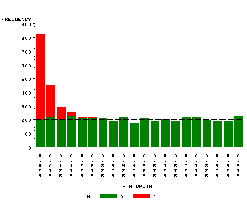
\epsfig{
%       file=.../Figures/HistoPvalRef.ps,
%       height=8cm, width=8cm, bbllx=82, bblly=304, bburx=277,
%       bbury=460, angle=90, clip=} 
  \end{tabular}
\end{tabular}
$$
\begin{tabular}{ll}
  \paragraph{$a$:} & the proportion of differentially expressed genes
  \\
  \paragraph{$f$:} & the  (alternative) density $f$ \\
\end{tabular}
$$

\newpage
\paragraph{Generalization:} We consider an i.i.d. sample $\{X_1,
\dots, X_n\}$ with mixture density
$$
g(x) = a f(x) + (1-a) \phi(x)
$$
\begin{tabular}{lr}
  The proportion $a$ is unknown &  $\longrightarrow$ \paragraph{parametric part} \\ 
  \\
  The density $f$ is completely unknown & \quad $\longrightarrow$ \paragraph{non
    parametric part} \\ 
  \\
  The density $\phi$ in completely specified & ($\Ucal_{[0, 1]}$,
  $\Ncal(0, 1)$, {\it etc.})
\end{tabular}

\bigskip \bigskip
\paragraph{Posterior probability.} We are interested in the
estimation of 
$$
\tau_i = \Pr\{Z_i = 1 \;|\; x_i\} = \Esp(Z_i \;|\; x_i) = \frac{a
  f(x_i)}{g(x_i)}
$$
where $Z_i =
\left\{
\begin{tabular}{rll}
  $Z_i = 1$ & if $i$ comes from $f$ & ($\Hbf_0(i)$ false), \\
  \\
  $Z_i = 0$ & otherwise & ($\Hbf_0(i)$ true).
\end{tabular}
\right.$


%%%%%%%%%%%%%%%%%%%%%%%%%%%%%%%%%%%%%%%%%%%%%%%%%%%%%%%%%%%%%%%%%%%%%%
%%%%%%%%%%%%%%%%%%%%%%%%%%%%%%%%%%%%%%%%%%%%%%%%%%%%%%%%%%%%%%%%%%%%%%
\newpage
\section{Density estimation}

\hspace{-2cm}
\begin{tabular}{ll}
  \begin{tabular}{p{10cm}}
  \paragraph{Kernel estimate.} A natural non-parametric estimate of $f$
  is \\
  $\displaystyle{\widehat{f}(x) = \frac1{\sum_i Z_i} \sum_i Z_i k_i(x)}$ \\
  where \\
  $\displaystyle{k_i(x) = \frac1h k\left(\frac{x-x_i}h\right)}$  \\
  \\
  $k$ being a kernel, i.e. a symmetric density function with mean
  0. \\
  \\
  \end{tabular}
  &
  \begin{tabular}{c}
    \epsfig{file=../Figures/FigKernelEstim.eps, width=9cm, height=13cm,
    angle=90, clip=, bbllx=77, bblly=61, bburx=552, bbury=676}
  \end{tabular}
\end{tabular}

\vspace{-0.5cm}
\paragraph{Weighted kernel estimate.} Since the $Z_i$'s are unknown,
we propose to replace them by their conditional expectations:
$$
\widehat{f}(x) = \frac1{\sum_i \tau_i}\sum_i \tau_i k_i(x)
$$
$\tau_i$ is the weight of observation $i$ in the estimation of $f$.
\newpage
\paragraph{Property of the $\widehat{\tau}_i$}. The estimates of the
$\tau_i$'s must satisfy
$$
\widehat{\tau}_j = \frac{a \widehat{f}(x_j)}{\widehat{g}(x_j)} 
= \frac{a \sum_i \widehat{\tau}_i k_i(x_j)}{a \sum_i \widehat{\tau}_i
  k_i(x_j) + (1-a) \phi(x_j) \sum_i \widehat{\tau}_i}
$$
or 
$$
\widehat{\tau}_j =\frac{\sum_i \widehat{\tau}_i b_{ij}}{\sum_i \widehat{\tau}_i b_{ij}
  + \sum_i \widehat{\tau}_i}
\qquad \mbox{with} \qquad
b_{ij} = \frac{a}{1-a} \frac{k_i(x_j)}{\phi(x_j)} \geq 0
$$

\paragraph{Function $\psibf$.}
$$
\begin{array}{rcl}
  \psibf: \Rbb^n & \rightarrow & \Rbb^n \\
  \ubf & \rightarrow &  \displaystyle{\psibf(\ubf): \psi_j(\ubf) = \frac{\sum_i
  u_i b_{ij}}{\sum_i u_i b_{ij}+ \sum_i u_i}}  
\end{array}
$$

\bigskip \bigskip 
\centerline{\fbox{$\widehat{\taubf} = (\widehat{\tau}_1, \dots,
  \widehat{\tau}_n)$ is a fixed point of $\psibf$.}}

\newpage
\paragraph{Estimation algorithm of $\taubf$.} Given some initial
$\widehat{\taubf}^{0}$, iterate $\psibf$:
$$
\widehat{\taubf}^{h+1} = \psibf(\widehat{\taubf}^{h}).
$$

\paragraph{$a$ remains fix:} it has to be estimated independently.

\paragraph{2 steps of the algorithm:} Connexion with E-M \\
{\bf ''E'' step:} given $\widehat{f}^h$ and $\widehat{g}^h$, calculate
$$
\widehat{\taubf}^{h+1} = a \widehat{f}^h(x_i) \left/
  \widehat{g}^h(x_i) \right..
$$
{\bf Other step:} given $\widehat{\taubf}^{h}$, estimate $f$ and
$g$:
$$
\widehat{f}^h(x) = \sum_i \widehat{\tau}^h_i k_i(x) \left/ \sum_i
  \widehat{\tau}^h_i \right., 
\qquad 
\widehat{g}^h(x) = a \widehat{f}^h(x) + (1-a) \phi(x).
$$
This second step does not maximize the likelihood $\longrightarrow$
not an E-M algorithm.

\newpage
\centerline{\framebox{
    \begin{tabular}{rl}
      \paragraph{Theorem:} & $\psibf$ is contracting \\
      \\
      $\Longrightarrow$ & the algorithm converges toward its unique
      fix point. 
    \end{tabular}
    }}

\paragraph{Sketch of proof.} $\psibf = \alphabf \circ \betabf \circ
\gammabf$:
$$
\alpha_j(\ubf) = \frac{u_j}{u_j + 1}, 
\qquad
\beta_j(\ubf) = \sum_i b_{ij} u_i, 
\qquad 
\gamma_j(\ubf) = \frac{u_j}{\sum_i u_i},
$$

\begin{description}
\item[1.] Brouwer's theorem: $\Ecal$ is compact and $\gammabf \circ
  \psibf$ is continuous, so at least one fix point exists. \\
\item[2.] Simplex $\Ecal = \{\ubf: \sum_i u_i = 1\}$ ($\gammabf = $
  projection on $\Ecal$)
  $$
  \ubf^* \in \Rbb^n: \psibf(\ubf) = \ubf
  \qquad \Longleftrightarrow \qquad
  \vbf^* = \gammabf(\ubf^*) \in \Ecal: \gammabf \circ \psibf (\vbf) = \vbf
  $$
  $\rightarrow$ Just consider $\gammabf \circ \psibf$ on the
  simplex $\Ecal$.
\end{description}

\newpage
\begin{description}
\item[3.] Interior of $\Ecal$: $\Ecal' = \{\ubf \in \Ecal: \forall i, u_i
  > 0\}$. 
  $$
  d(\ubf, \vbf) = \log \left[ \max_i \left(u_i / v_i\right)
    \left/ \min_i \left(u_i / v_i\right) \right. \right]
  $$
  is a distance on $\Ecal'$. %\\
\item[4.] $d$ decreases when $\psibf$ is applied:
  $$d[\gammabf \circ \psibf(\ubf), \gammabf \circ
  \psibf(\vbf)] < d(\ubf, \vbf)
  $$
  (except if $\ubf =  \vbf$). 
  $\rightarrow$ $\gammabf \circ \psibf$ admits at most one fix point
  in $\Ecal'$. %\\
\item[5.] If $k_{ij} > 0$ for all $(i, j)$: 
  $$
  \{\ubf \in \Ecal \setminus \Ecal'\} \quad \Longrightarrow \quad
  \{\gammabf \circ \psibf(\ubf) \in \Ecal'\}.
  $$
\end{description}
$\gammabf \circ \psibf$ (and therefore for $\psibf$) admits one unique
fix point toward which the algorithm converges.

%%%%%%%%%%%%%%%%%%%%%%%%%%%%%%%%%%%%%%%%%%%%%%%%%%%%%%%%%%%%%%%%%%%%%%
%%%%%%%%%%%%%%%%%%%%%%%%%%%%%%%%%%%%%%%%%%%%%%%%%%%%%%%%%%%%%%%%%%%%%%
\newpage
\section{Estimation of $a$ (and $h$)}

\paragraph{Analogy with EM. } $a$ could be estimated iteratively:
$$
\widehat{a}^h = \frac1n \sum_i \widehat{\tau}_i^h
$$
but
$$
\widehat{\taubf} = (\begin{array}{ccc}1 & \dots & 1 \end{array}), 
\qquad
\widehat{a} = 1
$$
is a fixed point of this algorithm.

\paragraph{Remark.} For a given $a$, there is a unique
$\widehat{\taubf}$. 

\bigskip\bigskip
\centerline{In some sense, $a$ is the unique parameter of the problem.}

%%%%%%%%%%%%%%%%%%%%%%%%%%%%%%%%%%%%%%%%%%%%%%%%%%%%%%%%%%%%%%%%%%%%%%
%%%%%%%%%%%%%%%%%%%%%%%%%%%%%%%%%%%%%%%%%%%%%%%%%%%%%%%%%%%%%%%%%%%%%%
\newpage
\paragraph{Empirical cdf.} The cumulative distribution function (cdf) of the
$p$-value can be estimated via its empirical version:
$$
\widehat{G}(p) = \frac1n \sum_{i=1}^n \Indic\{P_i \leq p\}.
$$
The cdf of the negative $p$-values is given by the uniform
distribution:
$$
\Pr\{P_i \leq p \;|\; i \in \Hbf_0\} = p.
$$

\paragraph{Cdf mixture.} Denoting $F$ the cdf of the positive
$p$-value, we have
$$
G(p) = a F(p) + (1-a) p.
$$
Above a certain threshold $t$, $F(p)$ should be close to 1: 
$$
x > t: \quad G(p) \simeq a + (1-a) p.  
$$

\newpage 
\paragraph{Empirical proportion.} Storey \& al, Genovese \& Wasserman
(JRSS-B, 02) propose an estimate of $a$ based on this approximation: 
$$
\widehat{a} = [1 - R(t)/n] / (1-t).
$$

\paragraph{Linear regression.}
$(1-a)$ can also be estimated by the coefficient of the linear
regression of $\widehat{G}(p)$ wrt $p$
$$
\epsfig{file=../Figures/RegGenoWas.eps, width=9cm, height=23cm, clip=, angle=90} 
$$


\newpage
\section{Estimation of $a$}

\paragraph{50 simulations.} 

\begin{center}
  \begin{tabular}{ccc}
    & Linear regression ($t = 1/2$) & Cross-validation ($\max_a
    \Lcal_{CV}$) \\
    \\
    \begin{rotate}{90}{\hspace{4cm}$(\widehat{a} - a)$}\end{rotate}
    &
    \epsfig{file= /RECHERCHE/EXPRESSION/COMPMULT/EMpondere/ADinit.ps,
      bbllx=52, bblly=52, bburx=560, bbury=710, clip=, width=10cm,
      height=10cm}
    & 
    \epsfig{file= /RECHERCHE/EXPRESSION/COMPMULT/EMpondere/ADmax.ps,
      bbllx=52, bblly=52, bburx=560, bbury=710, clip=, width=10cm,
      height=10cm} \\
    & $a$ & $a$
  \end{tabular}
\end{center}

% \newpage
% \paragraph{Cross-validation.} $h$ can also be estimated as follows
% \begin{enumerate}
% \item Split the dataset $\Dcal$ into $V$ subsets $\Dcal_1, \dots,
%   \Dcal_V$. \\
%   Typically, $V = 5$ or $10$. \\
% \item For $v=1 \dots V$
%   \begin{itemize}
%   \item estimate $f$ and $g$ with the data from $\Dcal \setminus
%     \Dcal_v$ ($\rightarrow \widehat{f}_v, \widehat{g}_v$), \\
%   \item calculate
%     $$
%     \Lcal_{CV}(\Dcal; a) = \frac1V \sum_v \sum_{i \in \Dcal_v} \log
%     \widehat{g}_v(x_i).
%     $$
%     \end{itemize}
%   \item Maximize $\Lcal_{CV}$ (numerically):
%     $$
%     \widehat{a} = \arg\max_a \Lcal_{CV}(\Dcal; a).
%     $$
% \end{enumerate}

%%%%%%%%%%%%%%%%%%%%%%%%%%%%%%%%%%%%%%%%%%%%%%%%%%%%%%%%%%%%%%%%%%%%%%
%%%%%%%%%%%%%%%%%%%%%%%%%%%%%%%%%%%%%%%%%%%%%%%%%%%%%%%%%%%%%%%%%%%%%%
\newpage
\section{Estimation of the $FDR$ (and $FNR$)}
\bigskip

\paragraph{Definition.} Recall that, when the $i$ tests with smallest
$p$-values are declared positive ($t = P_{(i)}$, $R(t) = i$):
$$
FDR_{(i)} = \Esp[FP(t) / i], 
\qquad 
FNR_{(i)} = \Esp[FN(t) / (1-i+1)]
$$
These definitions may be rephrased in terms of mixture model:
$$
FDR_{(i)} = \frac1i \sum_{j: P_j \leq P_{(i)}} (1-\tau_j), 
\qquad
FNR_{(i)} = \frac1{n-i+1} \sum_{j: P_j \leq P_{(i)}} \tau_j.
$$
The local $FDR$ is $\lFDR_{i} = 1-\tau_{i}$.

\bigskip\bigskip
\paragraph{Estimation.} We get the natural estimates:
$$
\widehat{FDR}_{(i)} = \frac1i \sum_{j \leq i} (1-\widehat{\tau}_j), 
\qquad
\widehat{FNR}_{(i)} = \frac1{n-i+1} \sum_{j > i} \widehat{\tau}_j,
\qquad
\widehat{\lFDR}{i} = 1-\widehat{\tau}_{i}.
$$

%%%%%%%%%%%%%%%%%%%%%%%%%%%%%%%%%%%%%%%%%%%%%%%%%%%%%%%%%%%%%%%%%%%%%%
%%%%%%%%%%%%%%%%%%%%%%%%%%%%%%%%%%%%%%%%%%%%%%%%%%%%%%%%%%%%%%%%%%%%%%
%%%%%%%%%%%%%%%%%%%%%%%%%%%%%%%%%%%%%%%%%%%%%%%%%%%%%%%%%%%%%%%%%%%%%%
%%%%%%%%%%%%%%%%%%%%%%%%%%%%%%%%%%%%%%%%%%%%%%%%%%%%%%%%%%%%%%%%%%%%%%
\newpage
\chapter{Applications}
\bigskip
%%%%%%%%%%%%%%%%%%%%%%%%%%%%%%%%%%%%%%%%%%%%%%%%%%%%%%%%%%%%%%%%%%%%%%
%%%%%%%%%%%%%%%%%%%%%%%%%%%%%%%%%%%%%%%%%%%%%%%%%%%%%%%%%%%%%%%%%%%%%%
\section{Probit transform}
%Instead of modeling the distribution of the $P_i$', we consider the
%$$
\begin{tabular}{lcr}
  $P_i \in [0, 1]$
  &   
  \qquad 
  &
  $X_i = \Phi^{-1}(P_i) \in \Rbb$ 
  \\
  \multicolumn{3}{c}{(Efron, JASA, 2005)}
  \\
  \textred{$\phi = \Ucal_{[0; 1]}$}
  & 
  & 
  \textred{$\phi = \Ncal(0, 1)$}
  \\
  \\
  \\
  \epsfig{figure=../Figures/HistoPval.ps, height=8cm, width=11.5cm,
    clip=, bbllx=26, bblly=40, bburx=176, bbury=130}   
  &
  &
%  \vspace{-2cm}
  \epsfig{figure=../Figures/HistoProbit.ps, height=8cm, width=11.5cm,
    clip=, bbllx=26, bblly=39, bburx=176, bbury=130}   
\end{tabular}
%$$

%%%%%%%%%%%%%%%%%%%%%%%%%%%%%%%%%%%%%%%%%%%%%%%%%%%%%%%%%%%%%%%%%%%%%%
%%%%%%%%%%%%%%%%%%%%%%%%%%%%%%%%%%%%%%%%%%%%%%%%%%%%%%%%%%%%%%%%%%%%%%
\newpage
\section{Cross-validation estimation of $h$ (and $a$)}

\paragraph{Hedenfalk data.} Comparison of 2 breast cancers (BRCA1 /
BRCA2): \\
$n = 3226$ genes, Epanechnikov kernel, Cochran test %(t-test with heterogenous group variances)

\bigskip\bigskip \hspace{-2cm}
\begin{tabular}{c@{}c@{}c} 
  \multicolumn{2}{c}{log-likelihood $\Lcal(a, h)$, \quad ($V = 5$)} \\
  \\
  training set & test set: $\Lcal_{CV}$ \\
  \begin{tabular}{c}
    \epsfig{
      file=/RECHERCHE/EXPRESSION/EXEMPLES/HEDENFALK/Amax/Asup-0.8/Cochran-Gaus.eps,
      height=8cm, width=8cm, bbllx=330, bblly=500, bburx=550,
      bbury=710, clip=, angle=90} 
  \end{tabular}
  &
  \begin{tabular}{c} 
    \epsfig{
      file=/RECHERCHE/EXPRESSION/EXEMPLES/HEDENFALK/Amax/Asup-0.8/Cochran-Gaus.eps,
      height=8cm, width=8cm, bbllx=330, bblly=290, bburx=550,
      bbury=500, clip=, angle=90} 
  \end{tabular}
  &
  \begin{tabular}{c} 
    \epsfig{
      file=/RECHERCHE/EXPRESSION/EXEMPLES/HEDENFALK/Amax/Asup-0.8/Cochran-Gaus.eps,
      height=8cm, width=8cm, bbllx=330, bblly=80, bburx=555,
      bbury=290, clip=, angle=90} 
  \end{tabular}
  \\
  $\widehat{a} \rightarrow 1, \quad \widehat{h} \rightarrow 0$
  & $\widehat{h} = 0.177$
  & $\widehat{a} = 0.443$
\end{tabular}


%%%%%%%%%%%%%%%%%%%%%%%%%%%%%%%%%%%%%%%%%%%%%%%%%%%%%%%%%%%%%%%%%%%%%%
%%%%%%%%%%%%%%%%%%%%%%%%%%%%%%%%%%%%%%%%%%%%%%%%%%%%%%%%%%%%%%%%%%%%%%
\newpage
\section{Hedenfalk data}

\paragraph{Student t-test} with homogenous variance $\sigma_i = $
cst. Gaussian kernel.

\hspace{-2cm}
\begin{tabular}{cc} 
  \begin{tabular}{c}
    $\widehat{a} = 20.6 \%$ \\
    $\textblue{\widehat{g}(x)}  = \widehat{a} \textred{\widehat{f}(x)} + (1-\widehat{a})
    \textgreen{\widehat{f}(x)}$ \\ 
    \epsfig{
      file=/RECHERCHE/EXPRESSION/EXEMPLES/HEDENFALK/Ainit/Asup-1.0/Homogen-Gaus.eps,
      height=12cm, width=9cm, bbllx=66, bblly=510, bburx=283,
      bbury=691, clip=, angle=90} 
  \end{tabular}
  &
  \begin{tabular}{c} 
    $\textred{\widehat{FDR}_i}, \textblue{\widehat{\tau}_i} \times
    \Phi^{-1}(P_i)$ \\ 
    \epsfig{
      file=/RECHERCHE/EXPRESSION/EXEMPLES/HEDENFALK/Ainit/Asup-1.0/Homogen-Gaus.eps,
      height=12cm, width=4.5cm, bbllx=66, bblly=295, bburx=283,
      bbury=480, clip=, angle=90} 
    \\
    $\textred{\widehat{FDR}_i}, \textblue{\widehat{\tau}_i} \times
    P_i$ \\ 
    \epsfig{
      file=/RECHERCHE/EXPRESSION/EXEMPLES/HEDENFALK/Ainit/Asup-1.0/Homogen-Gaus.eps,
      height=12cm, width=4.5cm, bbllx=66, bblly=85, bburx=283,
      bbury=265, clip=, angle=90} 
  \end{tabular}
\end{tabular}

\noindent $\Hbf_0$ (negative) $p$-values are not uniformly distributed
over [0, 1]. \\
The non-parametric part $\widehat{f}$ captures this departure of the
null distribution.

\newpage
\paragraph{Variance modeling} $K = 5$ groups of variances.

\hspace{-2cm}
\begin{tabular}{cc} 
  \begin{tabular}{c}
    $\widehat{a} = 30.5 \%$ \\
    $\textblue{\widehat{g}(x)}  = a \textred{\widehat{f}(x)} + (1-a)
    \textgreen{\widehat{f}(x)}$ \\ 
    \epsfig{
      file=/RECHERCHE/EXPRESSION/EXEMPLES/HEDENFALK/Ainit/Asup-1.0/Varmixt-Gaus.eps,
      height=12cm, width=9cm, bbllx=66, bblly=510, bburx=283,
      bbury=691, clip=, angle=90} 
  \end{tabular}
  &
  \begin{tabular}{c} 
    $\textred{\widehat{FDR}_i}, \textblue{\widehat{\tau}_i} \times
    \Phi^{-1}(P_i)$ \\ 
    \epsfig{
      file=/RECHERCHE/EXPRESSION/EXEMPLES/HEDENFALK/Ainit/Asup-1.0/Varmixt-Gaus.eps,
      height=12cm, width=4.5cm, bbllx=66, bblly=295, bburx=283,
      bbury=480, clip=, angle=90} 
    \\
    $\textred{\widehat{FDR}_i}, \textblue{\widehat{\tau}_i} \times
    P_i$ \\ 
    \epsfig{
      file=/RECHERCHE/EXPRESSION/EXEMPLES/HEDENFALK/Ainit/Asup-1.0/Varmixt-Gaus.eps,
      height=12cm, width=4.5cm, bbllx=66, bblly=85, bburx=283,
      bbury=265, clip=, angle=90} 
  \end{tabular}
\end{tabular}

\centerline{$
  \begin{array}{ccccc}
    \quad \widehat{FDR}_{(i)} \quad & \qquad i \qquad & \quad P_{(i)}
    \quad & \quad \widehat{\tau}_{(i)} \quad & \quad
    \widehat{FNR}_{(i)} \quad \\  
    \hline
    1\% & 4 & 2.5\;10^{-5} & 0.988 & 31.5 \% \\
    5\% & 142 & 3.1\;10^{-3} & 0.914 & 28.7 \% \\
    10\% & 296 & 1.3\;10^{-2} & 0.798 & 25.7 \% \\
  \end{array}
$}
\vspace{-0.5cm}
$\widehat{FDR}_{(i)} = \widehat{FNR}_{(i)} = 19.7 \%$ for $(i) = 633,
P_{(i)} = 5.4 \%, \widehat{\tau}_{(i)} = 43.5 \%$.

%%%%%%%%%%%%%%%%%%%%%%%%%%%%%%%%%%%%%%%%%%%%%%%%%%%%%%%%%%%%%%%%%%%%%%
%%%%%%%%%%%%%%%%%%%%%%%%%%%%%%%%%%%%%%%%%%%%%%%%%%%%%%%%%%%%%%%%%%%%%%
%%%%%%%%%%%%%%%%%%%%%%%%%%%%%%%%%%%%%%%%%%%%%%%%%%%%%%%%%%%%%%%%%%%%%%
%%%%%%%%%%%%%%%%%%%%%%%%%%%%%%%%%%%%%%%%%%%%%%%%%%%%%%%%%%%%%%%%%%%%%%
\end{document}
%%%%%%%%%%%%%%%%%%%%%%%%%%%%%%%%%%%%%%%%%%%%%%%%%%%%%%%%%%%%%%%%%%%%%%
%%%%%%%%%%%%%%%%%%%%%%%%%%%%%%%%%%%%%%%%%%%%%%%%%%%%%%%%%%%%%%%%%%%%%%
%%%%%%%%%%%%%%%%%%%%%%%%%%%%%%%%%%%%%%%%%%%%%%%%%%%%%%%%%%%%%%%%%%%%%%
%%%%%%%%%%%%%%%%%%%%%%%%%%%%%%%%%%%%%%%%%%%%%%%%%%%%%%%%%%%%%%%%%%%%%%

